\documentclass[aspectratio=169,11pt]{beamer}
\usepackage[utf8]{inputenc}
\usepackage[T1]{fontenc}
\usepackage[spanish]{babel}
\usepackage{amsmath,amssymb}
\usepackage{tikz}
\usetikzlibrary{arrows.meta,angles,calc,positioning}
\usetheme{Madrid}
\usecolortheme{default}
\setbeamertemplate{navigation symbols}{}
\setbeamertemplate{blocks}[rounded][shadow=false]
\newcommand{\ang}[1]{\angle #1^\circ}

\title[QFT en control digital]{Paso 10: QFT en control digital}
\subtitle{El controlador es un programa: muestreo, retenedor y plano $w$}
\author{Curso de control robusto (QFT)}
\date{}
\begin{document}
\begin{frame}\titlepage\end{frame}

\begin{frame}{Dónde encaja este paso}
  \tiny
  \begin{enumerate}\setlength{\itemsep}{-2pt}
    \item[1.] Números complejos \hfill \textcolor{gray}{(hecho)}
    \item[2.] Funciones de transferencia: $s$, polos y ceros \hfill \textcolor{gray}{(hecho)}
    \item[3.] Respuesta en frecuencia: $s=j\omega$, magnitud y fase \hfill \textcolor{gray}{(hecho)}
    \item[4.] Decibelios y escala logarítmica (Bode) \hfill \textcolor{gray}{(hecho)}
    \item[5.] Realimentación: $L$, $T=\frac{L}{1+L}$, $S=\frac{1}{1+L}$ \hfill \textcolor{gray}{(hecho)}
    \item[6.] Nichols chart \hfill \textcolor{gray}{(hecho)}
    \item[7.] Incertidumbre y templates \hfill \textcolor{gray}{(hecho)}
    \item[8.] Especificaciones $\rightarrow$ bounds \hfill \textcolor{gray}{(hecho)}
    \item[9.] Loop shaping, prefiltro y verificación \hfill \textcolor{gray}{(hecho)}
    \item[\textbf{10.}] \textbf{QFT en control digital} \hfill $\leftarrow$ estamos aquí
    \item[11.] Dos caminos digitales: $z$ y $w$
    \item[12.] Estabilidad, límites, más especificaciones y caso real
    \item[13.] Muestreo por eventos con periodo base $T$
    \item[14.] Sistemas de dos estados: lazo interno y externo
    \item[15.] QFT y sistemas no lineales
    \item[16.] Algoritmos de QFT: cómo funcionan por dentro
    \item[17.] QFT en Python: una biblioteca paso a paso
    \item[18.] QFT en MATLAB: el mismo código, otra sintaxis
    \item[19.] Historia, panorama y bibliografía
  \end{enumerate}
  \vspace{2pt}
  \begin{block}{Objetivo de hoy}
    Ver qué cambia (y qué \textbf{no}) cuando $G$ y $F$ se ejecutan en un computador con periodo de muestreo $T_s$. Casi todo lo aprendido se conserva; cambia el eje de frecuencias y aparece un retardo.
  \end{block}
\end{frame}

\begin{frame}{El lazo con controlador digital}
  \small
  \begin{center}
  \begin{tikzpicture}[>=Stealth,every node/.style={font=\footnotesize}]
    \node (r) at (0,0) {$r$};
    \node[draw,minimum width=0.9cm,minimum height=0.65cm] (F) at (1.1,0) {$F(z)$};
    \node[draw,circle,inner sep=0.5pt] (sum) at (2.4,0) {$+$};
    \node[draw,minimum width=0.9cm,minimum height=0.65cm] (G) at (3.8,0) {$G(z)$};
    \node[draw,minimum width=0.9cm,minimum height=0.65cm] (zoh) at (5.5,0) {ZOH};
    \node[draw,minimum width=0.9cm,minimum height=0.65cm] (P) at (7.1,0) {$P(s)$};
    \node (y) at (8.8,0) {$y$};
    \node[draw,circle,inner sep=1.5pt] (S) at (7.6,-1.2) {};
    \draw[->] (r)--(F); \draw[->] (F)--(sum); \draw[->] (sum)--(G); \draw[->] (G)--(zoh); \draw[->] (zoh)--(P); \draw[->] (P)--(y);
    \draw[->] (8.1,0) |- (S.east); \draw[->] (S.west) -| node[pos=0.25,below]{$-1$} (sum.south);
    \node at (7.6,-1.65) {muestreo $T_s$};
  \end{tikzpicture}
  \end{center}
  \begin{itemize}
    \item $G(z)$, $F(z)$: algoritmos que se ejecutan cada $T_s$. Entre muestras la salida del DAC se mantiene constante: \textbf{retenedor de orden cero} (ZOH).
    \item $\omega_s=2\pi/T_s$ (frecuencia de muestreo); \textbf{frecuencia de Nyquist} $\omega_N=\pi/T_s$.
  \end{itemize}
\end{frame}

\begin{frame}{Qué se conserva y qué cambia}
  \small
  \begin{columns}[T]
  \begin{column}{0.48\textwidth}
    \begin{block}{Se conserva}
      \begin{itemize}
        \item La familia de plantas y los templates.
        \item Las especificaciones y los bounds.
        \item El Nichols chart y sus contornos de $|T|$.
        \item El loop shaping: sumar dB y grados.
      \end{itemize}
    \end{block}
  \end{column}
  \begin{column}{0.48\textwidth}
    \begin{block}{Cambia}
      \begin{itemize}
        \item El lazo se evalúa en $z=e^{j\omega T_s}$ en vez de $s=j\omega$.
        \item La planta ahora incluye ZOH: $P(z)=\mathcal{Z}\{\text{ZOH}\cdot P(s)\}$.
        \item Solo existe respuesta hasta $\omega_N$.
      \end{itemize}
    \end{block}
  \end{column}
  \end{columns}
  \begin{alertblock}{La idea}
    $L(e^{j\omega T_s})=G(z)\,P(z)\big|_{z=e^{j\omega T_s}}$ es un número complejo por frecuencia, exactamente como antes. Todo el método QFT se aplica sin tocar.
  \end{alertblock}
\end{frame}

\begin{frame}{De $s=j\omega$ a $z=e^{j\omega T_s}$}
  \footnotesize
  \centering
  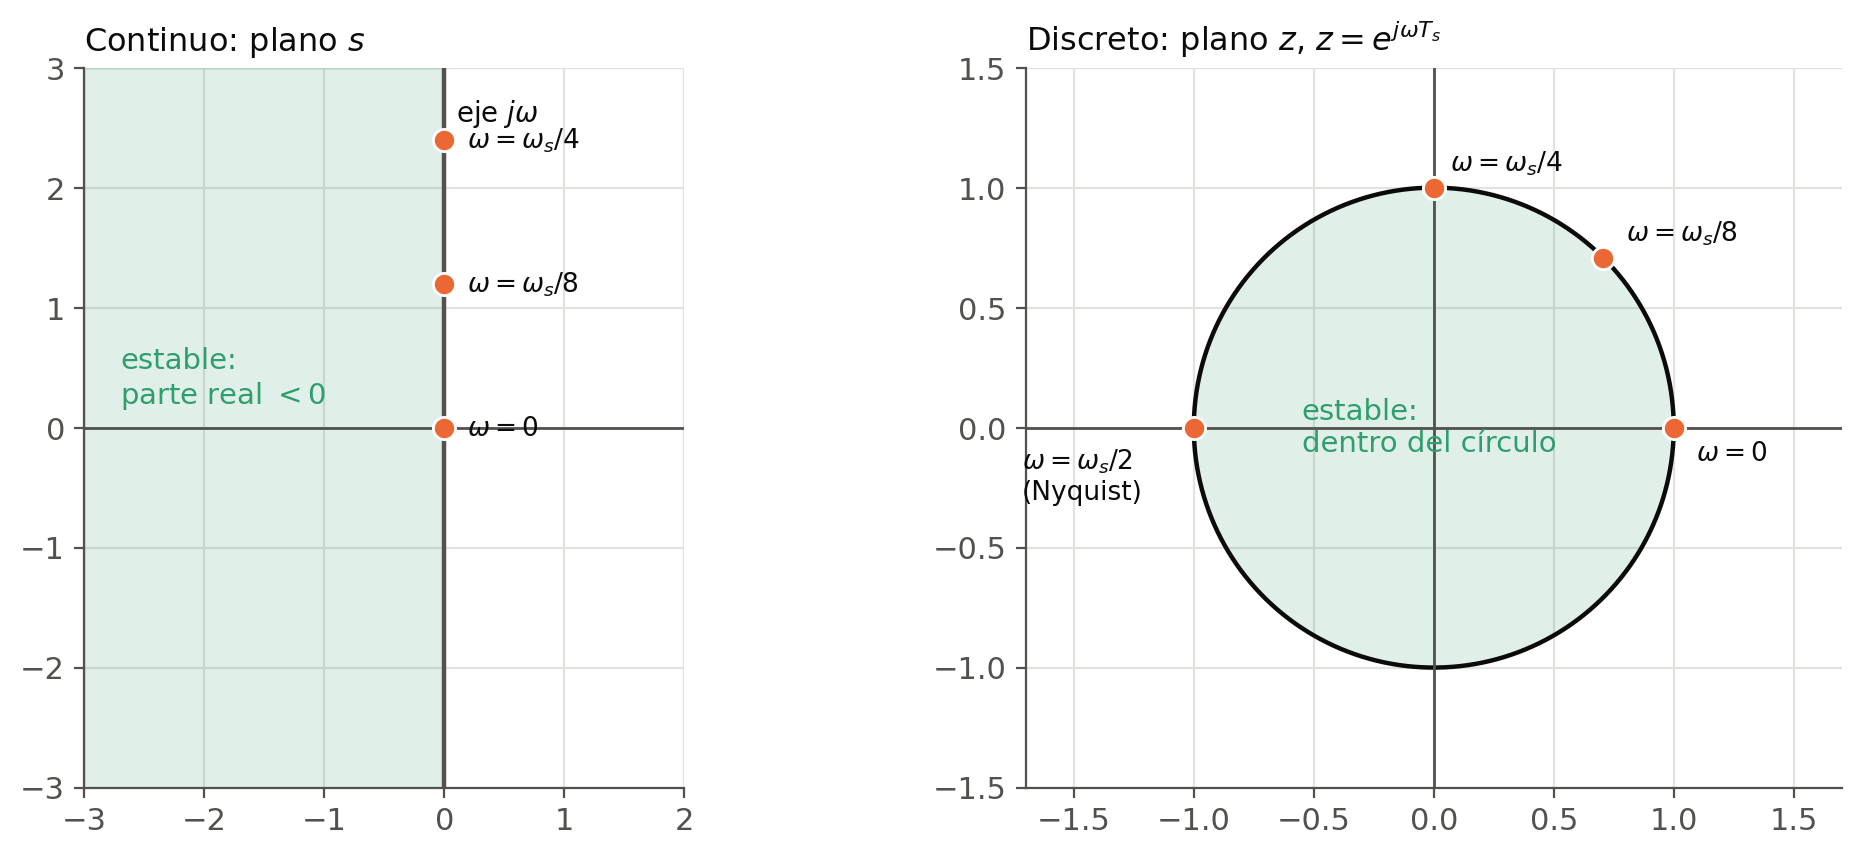
\includegraphics[width=0.85\textwidth]{fig/s_z.png}\\[2pt]
  \begin{columns}[T]
  \begin{column}{0.48\textwidth}
    El eje imaginario del plano $s$ se enrolla en la \textbf{circunferencia unidad}. La estabilidad pasa de ``parte real $<0$'' a ``polos dentro del círculo''.
  \end{column}
  \begin{column}{0.48\textwidth}
    La arista $z=-1$ es Nyquist. Más allá, la respuesta se repite (periódica en $\omega_s$). La flecha $(z-p)$ sigue siendo la del paso 2.
  \end{column}
  \end{columns}
\end{frame}

\begin{frame}{El ZOH es un retardo de $T_s/2$}
  \footnotesize
  \begin{columns}[T]
  \begin{column}{0.5\textwidth}
    $\mathrm{ZOH}(s)=\dfrac{1-e^{-sT_s}}{s}$. En $s=j\omega$:
    \[ \mathrm{ZOH}(j\omega)=T_s\,\underbrace{\frac{\sin(\omega T_s/2)}{\omega T_s/2}}_{\text{módulo}\ \approx1}\;e^{-j\omega T_s/2} \]
    \begin{itemize}
      \item Módulo: casi $1$ si $\omega\ll\omega_s$ ($-0.36$ dB con $\omega T_s/2=0.5$).
      \item Fase: $-\omega T_s/2$ rad, igual que un retardo de $T_s/2$ segundos.
    \end{itemize}
    \begin{block}{Es el paso 4}
      Un retardo no cambia el módulo y resta fase proporcional a $\omega$. Con $T_s=0.05$ s: $-14.3^\circ$ a $\omega=10$.
    \end{block}
  \end{column}
  \begin{column}{0.48\textwidth}
    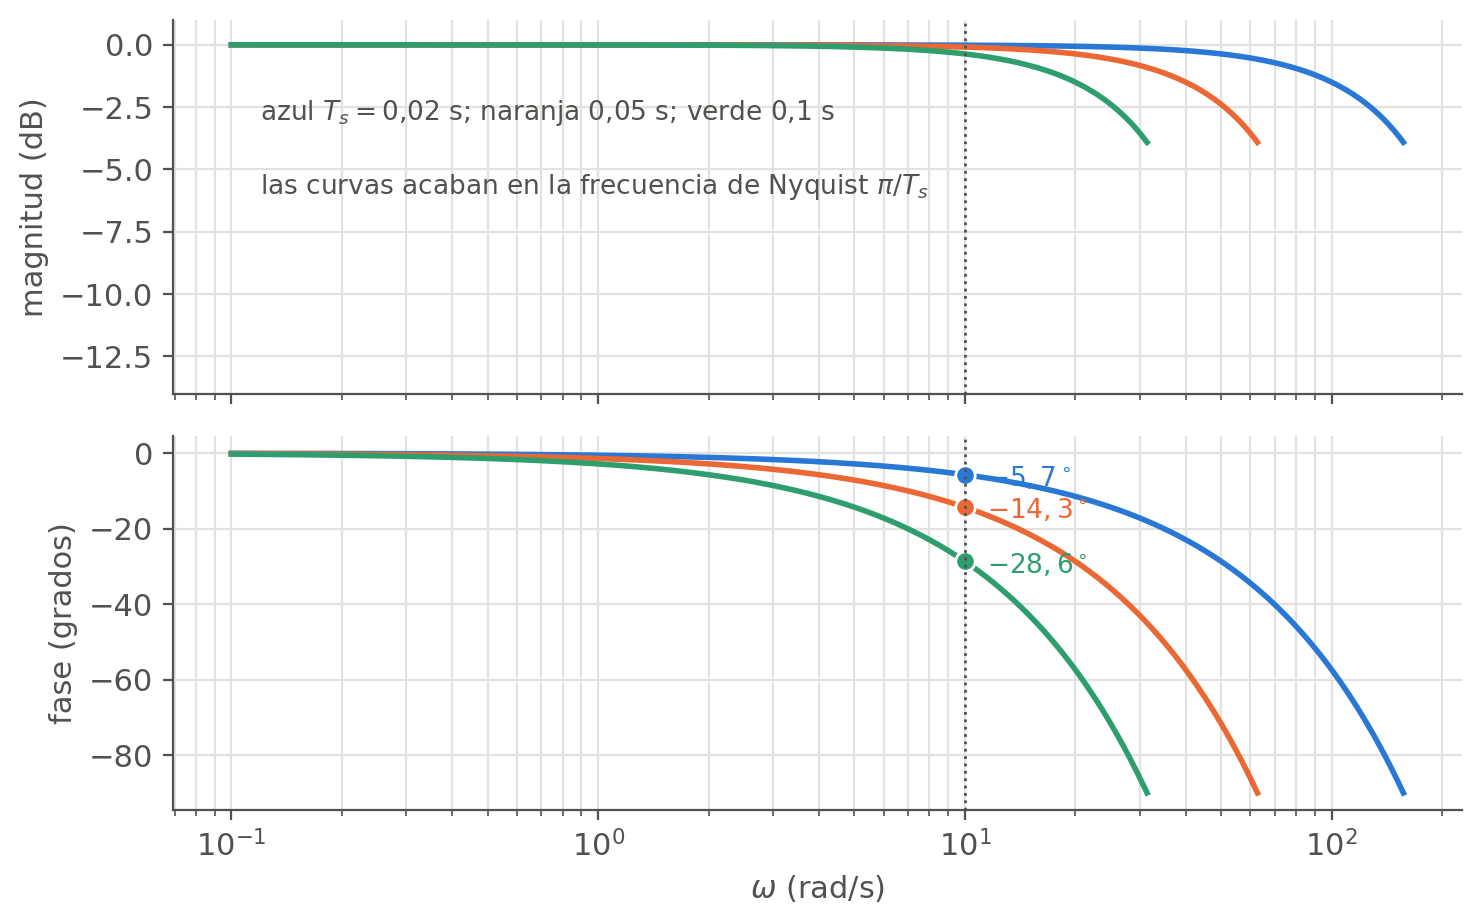
\includegraphics[width=\textwidth]{fig/zoh.png}
  \end{column}
  \end{columns}
\end{frame}

\begin{frame}{En el Nichols: la curva se desplaza a la izquierda}
  \footnotesize
  \begin{columns}[T]
  \begin{column}{0.64\textwidth}
    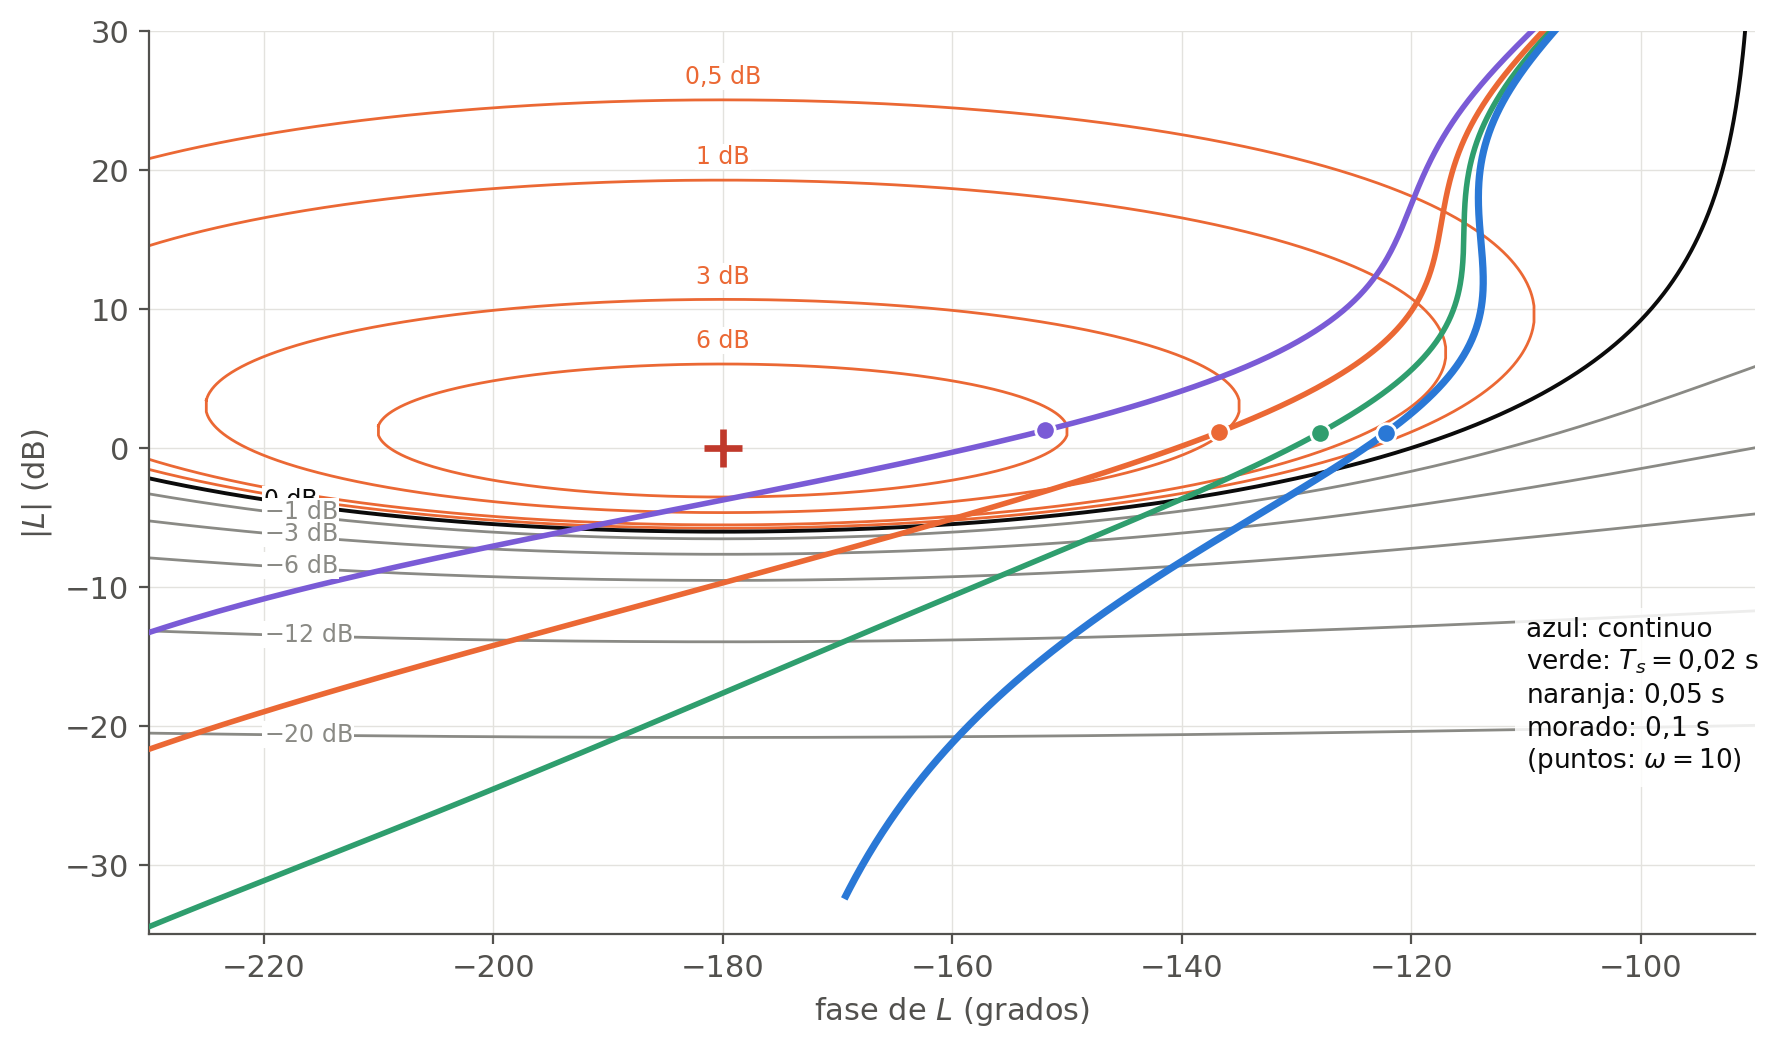
\includegraphics[width=\textwidth]{fig/nichols_dig.png}
  \end{column}
  \begin{column}{0.34\textwidth}
    Peor planta ($K=5$, $a=1$) con el $G$ del paso 9 pasado a digital por Tustin.
    \begin{itemize}
      \item En $\omega=10$ (puntos) la fase pasa de $-122^\circ$ (continuo) a $-128^\circ$, $-137^\circ$ y $-152^\circ$ con $T_s=0.02$, $0.05$ y $0.1$ s.
      \item La curva se acerca al punto crítico y entra en contornos de $|T|$ cada vez más altos.
    \end{itemize}
  \end{column}
  \end{columns}
\end{frame}

\begin{frame}{Los templates también se desplazan}
  \footnotesize
  \begin{columns}[T]
  \begin{column}{0.54\textwidth}
    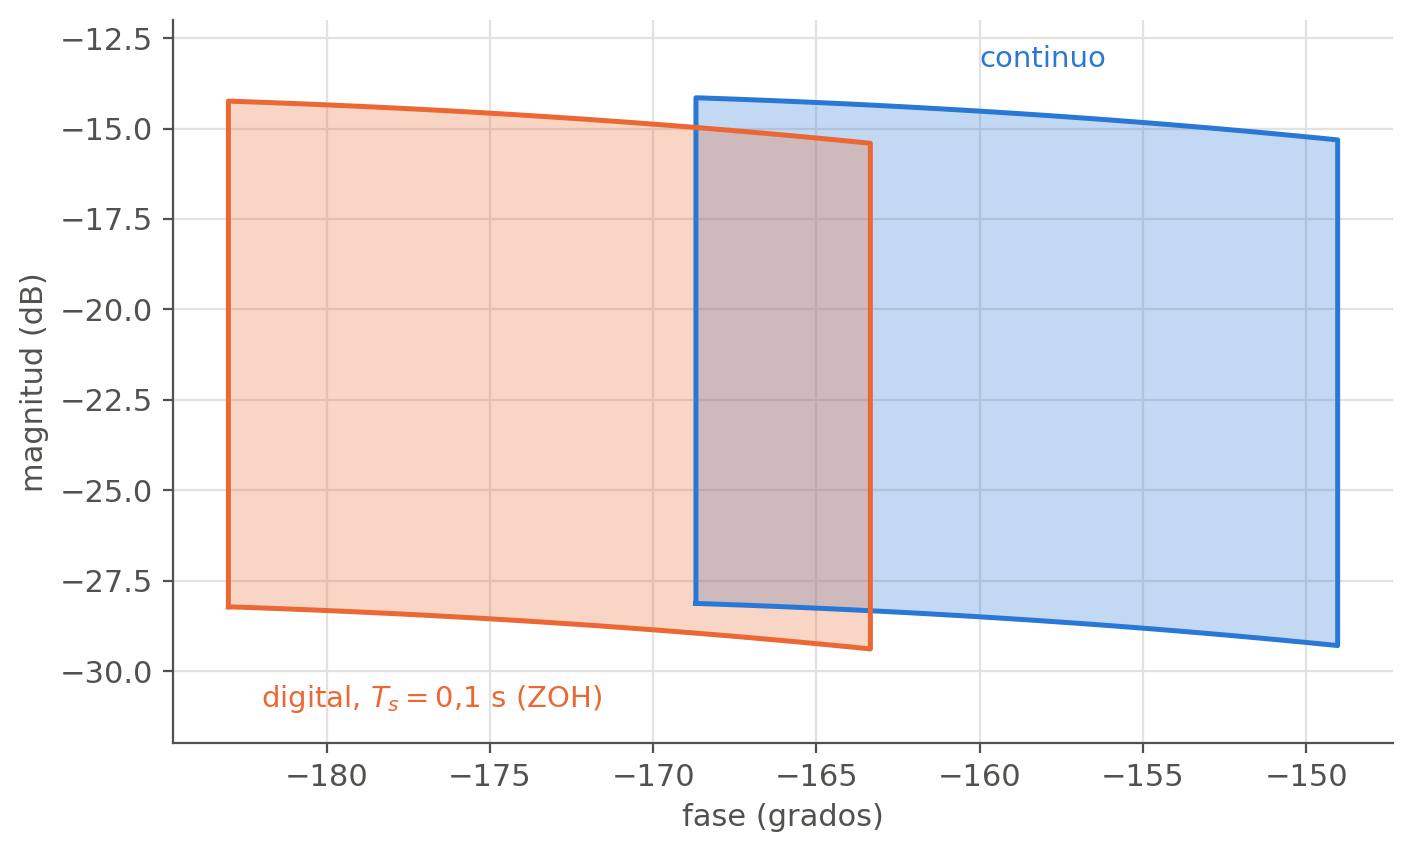
\includegraphics[width=\textwidth]{fig/template_dig.png}
  \end{column}
  \begin{column}{0.44\textwidth}
    Template en $\omega=5$ con $T_s=0.1$ s: se desplaza $\approx-14.3^\circ=-\omega T_s/2$ y casi no cambia de forma ni de dB ($-0.09$ dB).
    \begin{block}{Consecuencia}
      Las especificaciones y la forma del template siguen igual, pero el nominal que antes cumplía el bound ahora se queda corto de fase: hay que \textbf{compensar con más adelanto}.
    \end{block}
  \end{column}
  \end{columns}
\end{frame}

\begin{frame}{Cuánto cuesta un muestreo lento (con $G$ del paso 9 discretizado)}
  \small
  \begin{center}
  \begin{tabular}{c|c|c|c|c}
    $T_s$ (s) & $\omega_s/10$ & fase perdida en $\omega=10$ & $\max|T|$ & cumple $\le1.58$ dB\\\hline
    continuo & -- & -- & $0.94$ dB & sí\\
    $0.005$ & $126$ & $1.4^\circ$ & $1.06$ dB & sí\\
    $0.01$ & $63$ & $2.9^\circ$ & $1.21$ dB & sí\\
    $0.02$ & $31$ & $5.7^\circ$ & $1.59$ dB & al límite\\
    $0.05$ & $12.6$ & $14.3^\circ$ & $3.51$ dB & no\\
    $0.1$ & $6.3$ & $28.6^\circ$ & $10.0$ dB & no\\
    $0.15$ & $4.2$ & $43.0^\circ$ & $32.2$ dB & no
  \end{tabular}
  \end{center}
  \begin{alertblock}{Regla práctica}
    Para que el ZOH cueste pocos grados, $\omega_s\gtrsim30$ veces el ancho de banda del lazo. Aquí $\omega_c\approx10$ rad/s $\Rightarrow$ $T_s\lesssim0.02$ s.
  \end{alertblock}
\end{frame}

\begin{frame}{Cómo se nota en el tiempo}
  \footnotesize
  \begin{columns}[T]
  \begin{column}{0.6\textwidth}
    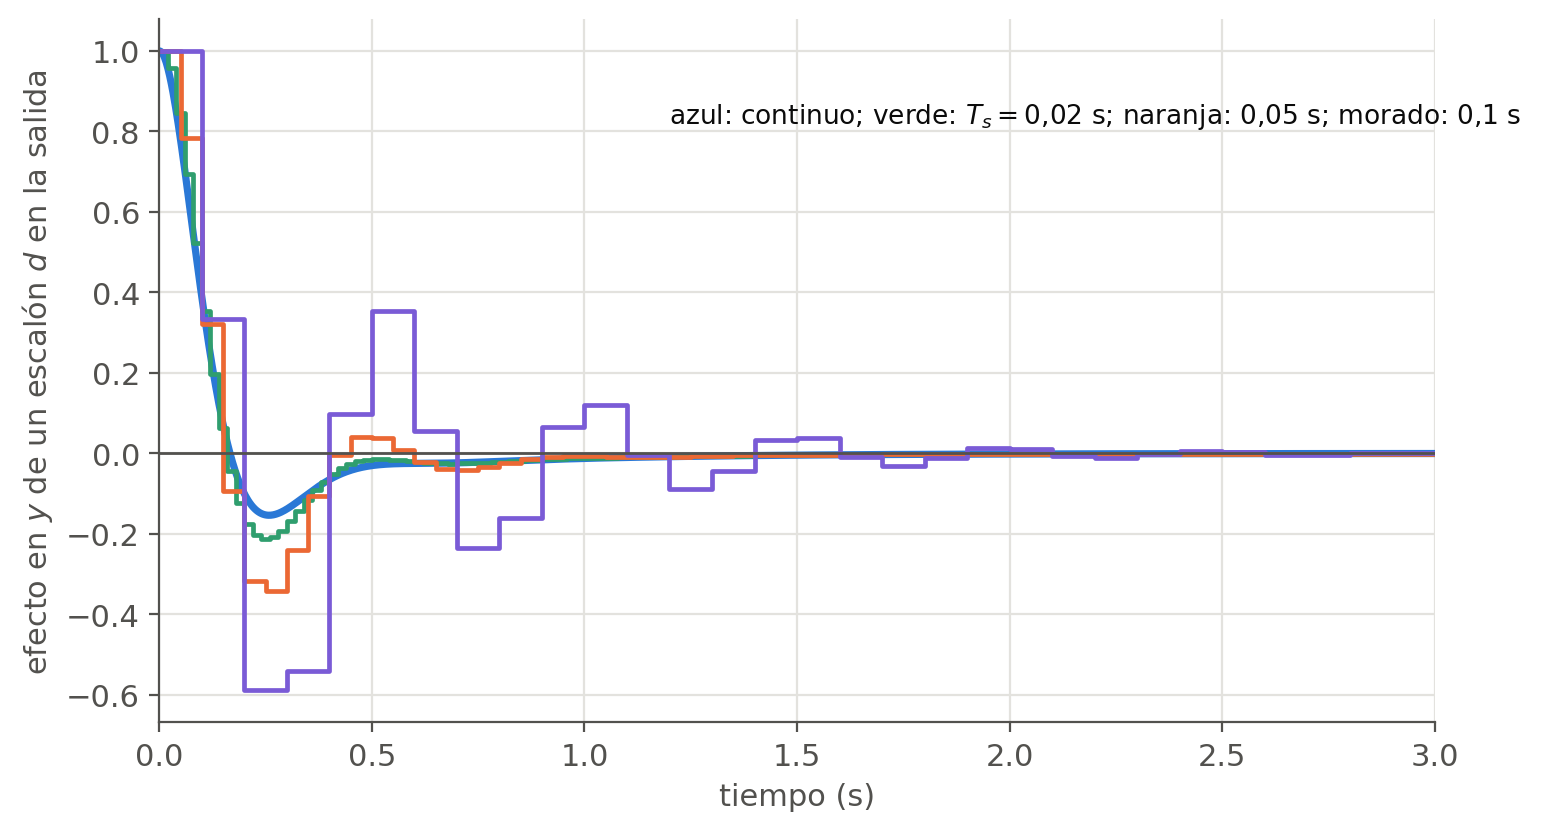
\includegraphics[width=\textwidth]{fig/escalon_dig.png}
  \end{column}
  \begin{column}{0.38\textwidth}
    Respuesta de la salida a un escalón de perturbación $d$ en la salida ($y/d=S$) para la peor planta:
    \begin{itemize}
      \item Continuo: sub-oscilación de $-0.15$.
      \item $T_s=0.02$: $-0.21$. $T_s=0.05$: $-0.34$.
      \item $T_s=0.1$: $-0.59$ y oscilación que tarda más en apagarse.
    \end{itemize}
    Es el pico de $|S|$ y de $|T|$ que vimos en el Nichols, ahora en segundos.
  \end{column}
  \end{columns}
\end{frame}

\begin{frame}{Dos caminos para diseñar $G(z)$}
  \small
  \begin{block}{A. Emulación}
    Diseñar $G(s)$ como en los pasos anteriores y discretizar (Tustin: $s\to\frac{2}{T_s}\frac{z-1}{z+1}$). Rápido, pero el retardo del ZOH no estaba en el diseño: hay que dejar \textbf{margen extra} o muestrear rápido.
  \end{block}
  \begin{block}{B. Diseño directo en discreto}
    Calcular templates con $P_i(z)$ (ya con ZOH), bounds con $L=G(z)P(z)$ en $z=e^{j\omega T_s}$, y hacer el loop shaping sobre esa curva. El retardo entra en el diseño desde el principio.
  \end{block}
  \begin{alertblock}{En la práctica}
    Se empieza por A (si $T_s$ es pequeño basta) y se pasa a B si el margen se agota. La verificación final siempre se hace con el lazo discreto.
  \end{alertblock}
\end{frame}

\begin{frame}{El plano $w$: volver a las herramientas continuas}
  \footnotesize
  \begin{columns}[T]
  \begin{column}{0.54\textwidth}
    Transformación bilineal: $\ w=\dfrac{2}{T_s}\,\dfrac{z-1}{z+1}$. Con $z=e^{j\omega T_s}$:
    \[ w=j\nu,\qquad \nu=\frac{2}{T_s}\tan\frac{\omega T_s}{2} \]
    \begin{itemize}
      \item El semiplano izquierdo de $w$ equivale al interior del círculo: la estabilidad vuelve a ser ``parte real $<0$''.
      \item $P(w)$ y $G(w)$ son racionales: Bode, Nichols y loop shaping se hacen como en el continuo.
      \item $\nu\approx\omega$ para $\omega T_s$ pequeño; cerca de Nyquist $\nu\to\infty$.
      \item El ZOH aparece como un cero en el semiplano derecho, $w\approx2/T_s$, que resta fase $\arctan(\nu T_s/2)=\omega T_s/2$.
    \end{itemize}
  \end{column}
  \begin{column}{0.44\textwidth}
    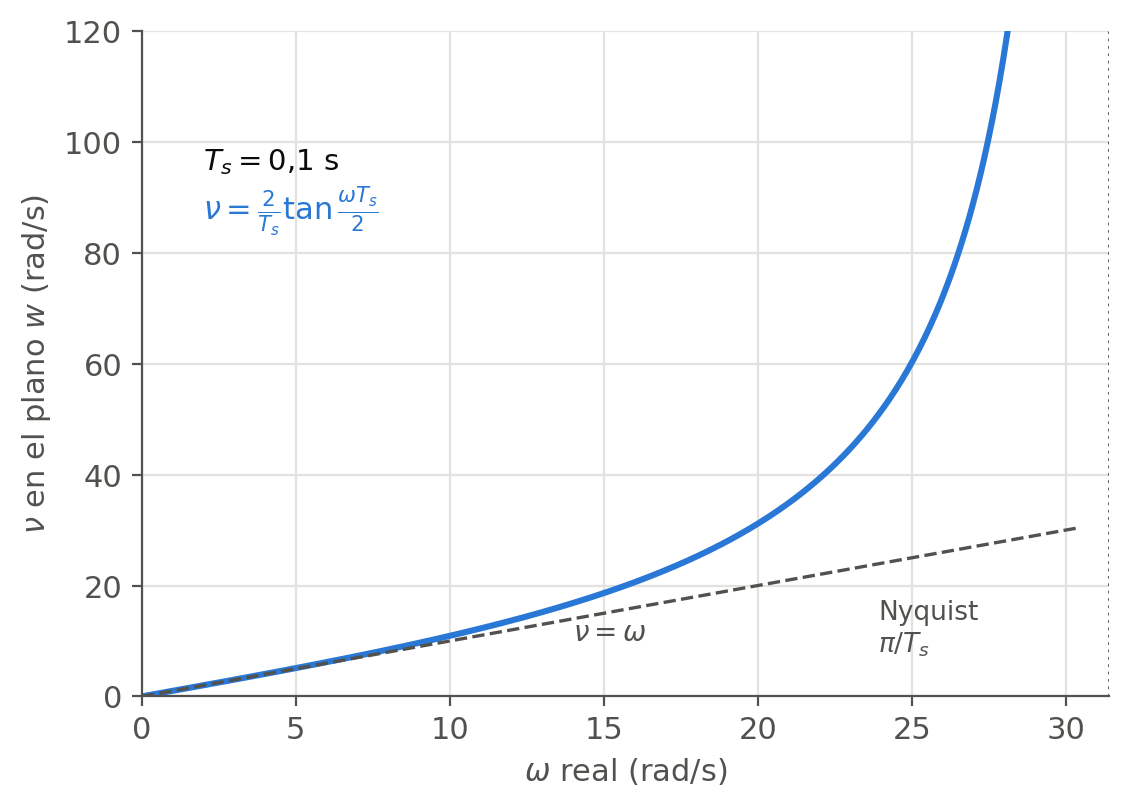
\includegraphics[width=\textwidth]{fig/plano_w.png}
  \end{column}
  \end{columns}
\end{frame}

\begin{frame}{Resultado del diseño directo con este ejemplo}
  \small
  Mismas especificaciones del paso 8, templates y bounds calculados con $P_i(z)$:
  \begin{center}
  \begin{tabular}{c|l|l}
    $T_s$ & Emulando el $G$ del paso 9 & Rediseñando el adelanto $G=k\frac{1+s/z}{1+s/p}$\\\hline
    $0.02$ & al límite ($1.59$ dB) & $k=5$, $z=2$, $p=25$: cumple\\[2pt]
    $0.05$ & incumple entre $\omega\approx6$ y $15$ ($3.51$ dB) & $k=5$, $z=2.3$, $p=32$: cumple (justo)\\[2pt]
    $0.1$ & incumple ($10$ dB) & no hay solución razonable con este tipo de $G$
  \end{tabular}
  \end{center}
  \begin{block}{Lectura}
    Subir el polo del adelanto (de $20$ a $32$) y mover el cero ($2\to2.3$) recupera fase con $T_s=0.05$ s (comprobado en una rejilla densa de frecuencias hasta Nyquist). Con $T_s=0.1$ s no hay compensador de adelanto sencillo que cumpla: o se baja $T_s$ o se relajan las especificaciones. \textbf{Hay un $T_s$ máximo} para cada especificación.
  \end{block}
\end{frame}

\begin{frame}{Implementación y trampas}
  \footnotesize
  \begin{columns}[T]
  \begin{column}{0.52\textwidth}
    $G(s)=\dfrac{50(s+2)}{s+20}$ con Tustin y $T_s=0.02$ s:
    \[ G(z)=\frac{42.5-40.83\,z^{-1}}{1-0.667\,z^{-1}} \]
    Es la ecuación en diferencias
    \[ u_k=0.667\,u_{k-1}+42.5\,e_k-40.83\,e_{k-1} \]
    ($e_k=$ error muestreado, $u_k=$ mando). El prefiltro $F=\frac{1.2}{s+1.2}$ da otra de primer orden.
  \end{column}
  \begin{column}{0.46\textwidth}
    \begin{alertblock}{Retardo de cómputo}
      Si $u_k$ se calcula con el dato $k$ pero se aplica en el periodo siguiente, el lazo suma otro retardo $T_s$ (fase $-\omega T_s$): en total $1.5\,T_s$ con el ZOH. Cuenta en el diseño.
    \end{alertblock}
    \begin{block}{Otras}
      \begin{itemize}
        \item Filtro anti-aliasing: resta fase propia.
        \item Saturación del actuador (anti-windup).
        \item Ruido: el $G(\infty)=50$ se aplica también al ruido de cuantización.
      \end{itemize}
    \end{block}
  \end{column}
  \end{columns}
\end{frame}

\begin{frame}{Ejercicio}
  \small
  Un lazo continuo tiene $\omega_c=10$ rad/s y margen de fase $56^\circ$. Se va a implementar con ZOH.
  \begin{enumerate}
    \item Con $T_s=0.1$ s, ¿qué retardo equivalente introduce el ZOH y cuánta fase resta en $\omega_c$? ¿Qué margen de fase queda (aproximadamente)?
    \item ¿Cuál es la frecuencia de Nyquist? ¿Está $\omega_c$ muy cerca?
    \item ¿Qué $T_s$ máximo permite perder como mucho $6^\circ$ de fase en $\omega_c$?
  \end{enumerate}
  \begin{block}{Pista}
    Retardo $T_s/2$ s $\Rightarrow$ fase $-\omega T_s/2$ rad $=-\frac{180}{\pi}\frac{\omega T_s}{2}$ grados.
  \end{block}
  \textcolor{gray}{Solución en el apéndice.}
\end{frame}

\begin{frame}{De dónde viene el QFT digital}
  \small
  \begin{itemize}
    \item Horowitz presentó en 1986 el desarrollo paralelo del QFT en el dominio discreto (plano $w$): se sustituye $s$ por $w\approx j\frac{2}{T}\tan\!\big(\frac{\omega_{sp}T}{2}\big)$.
    \item Detalle de diseños en Horowitz y Liao (1986a) y en Houpis y Lamont (1992).
    \item Idea clave de la literatura: \textbf{todo sistema muestreado es de fase no mínima}, lo que limita sus prestaciones frente al caso continuo; un buen diseño minimiza ese efecto.
  \end{itemize}
  \footnotesize Lo veremos con el retardo del ZOH y con el límite de $T_s$ en este paso y los siguientes.
\end{frame}

\begin{frame}{Para programarlo: el notebook de este paso}
  \small
  Todo lo de este paso se puede \textbf{ejecutar} en el notebook \texttt{notebooks/paso10\_digital.ipynb}.
  \begin{itemize}
    \item Python: el ZOH como retardo, $P(z)$ con \texttt{cont2discrete}, la tabla del coste de $T_s$ y el rediseño directo.
    \item Cada cálculo de las diapositivas se \textbf{comprueba} en código, con las mismas cifras.
    \item Incluye celdas \emph{Tu turno} con el ejercicio del paso y la solución plegada.
  \end{itemize}
  \footnotesize Requisitos: \texttt{numpy}, \texttt{scipy}, \texttt{matplotlib}; se abre con \texttt{jupyter lab notebooks/}. Ver \texttt{GUIA.md}.
\end{frame}

\begin{frame}{Resumen}
  \small
  \begin{itemize}
    \item Con controlador digital, el lazo se evalúa en $z=e^{j\omega T_s}$ hasta Nyquist $\pi/T_s$. Los templates, bounds y el Nichols se usan igual.
    \item El ZOH es un retardo de $T_s/2$: $-\omega T_s/2$ rad, módulo $\approx1$. Desplaza la curva y los templates a la izquierda.
    \item Emular un diseño continuo funciona si $\omega_s\gtrsim30\,\omega_c$; si no, rediseñar con el retardo incluido.
    \item El plano $w$ ($\nu=\frac{2}{T_s}\tan\frac{\omega T_s}{2}$) permite usar Bode y Nichols continuos para el diseño discreto.
    \item Hay un $T_s$ máximo por encima del cual las especificaciones ya no son alcanzables.
  \end{itemize}
\end{frame}

\appendix
\begin{frame}\centering\Large Apéndice\end{frame}

\begin{frame}{Solución del ejercicio}
  \small
  \textbf{1.} Retardo $T_s/2=0.05$ s. Fase: $-\omega_c T_s/2=-10\cdot0.05=-0.5$ rad $=-28.6^\circ$. Margen de fase: $56^\circ-28.6^\circ\approx27^\circ$ (aproximado: ignora el cambio de magnitud y la discretización de $G$).\\[3pt]
  \textbf{2.} $\omega_N=\pi/T_s=31.4$ rad/s. $\omega_c=10$ es un tercio de Nyquist: hay pocos puntos por periodo.\\[3pt]
  \textbf{3.} $\dfrac{180}{\pi}\dfrac{\omega_c T_s}{2}\le6^\circ\Rightarrow T_s\le\dfrac{2\cdot6\,\pi/180}{10}=0.0209$ s. Es el $T_s\lesssim0.02$ s de la tabla.
  \begin{block}{Con el retardo de cómputo}
    Si además se suma un periodo de retardo de cómputo, el límite pasa a $1.5\,T_s\,\omega_c\le6^\circ$, es decir $T_s\le0.007$ s.
  \end{block}
\end{frame}

\begin{frame}{Para curiosos: por qué el ZOH es un retardo}
  \small
  $\mathrm{ZOH}(s)=\dfrac{1-e^{-sT_s}}{s}$. Sacando factor común $e^{-sT_s/2}$:
  \[ 1-e^{-sT_s}=e^{-sT_s/2}\big(e^{sT_s/2}-e^{-sT_s/2}\big) \]
  \[ \Rightarrow\ \mathrm{ZOH}(j\omega)=e^{-j\omega T_s/2}\,\frac{2j\sin(\omega T_s/2)}{j\omega}=T_s\,\mathrm{sinc}\Big(\frac{\omega T_s}{2}\Big)e^{-j\omega T_s/2} \]
  \begin{block}{Interpretación}
    El módulo es un seno cardinal (cae suavemente hasta $2/\pi=-3.9$ dB en Nyquist) y la fase es la de un retardo puro de $T_s/2$. Al muestrear luego la salida de la planta, el factor $T_s$ se compensa con el $1/T_s$ del muestreador.
  \end{block}
\end{frame}
\end{document}
